\documentclass[10pt, a4paper]{article}
% The next line loads some packages you will need

\usepackage{graphicx, amsmath, amssymb, fancyhdr, setspace,titlesec,enumitem,indentfirst,hyperref}
\usepackage[labelfont=bf]{caption}
\usepackage[table]{xcolor}
\hypersetup{
    colorlinks=true,
    linkcolor=blue,
    filecolor=blue,      
    urlcolor=blue,
    pdftitle={Overleaf Example},
    pdfpagemode=FullScreen,
    }

% Page formatting
\addtolength{\textwidth}{5mm}
\addtolength{\textheight}{12mm}
\addtolength{\topmargin}{-10mm}
\pretolerance = 10000000
\setlength{\parindent}{23pt}
% \setlength{\parskip}{\baselineskip}
\onehalfspacing   

% Header / footer
\pagestyle{fancy}
\lhead{Himanshu Madan, 201501359}
\chead{}
\rhead{\em MATH 5747M, assignment 2}
\lfoot{}
\cfoot{\thepage}
\rfoot{}
\setlength{\headheight}{20pt}
\renewcommand{\headrulewidth}{0.4pt}
\renewcommand{\footrulewidth}{0pt}

% \titlespacing\section{0pt}{10pt plus 4pt minus 2pt}{0pt plus 0pt minus 0pt}

\begin{document}
\begin{center}
\textbf{\Large Decision Science Using MCDA} \\
Based on module LUBS 5308M Business Analytics and Decision Science \\
Lectured by Dr. Richard Hodgett \\
\end{center}

\section*{Introduction}
The objective of this report is to explain two different but prominent \textbf{Multi Criteria Decision Analysis} techniques:
\begin{itemize}[noitemsep]
    \item \textbf{Analytical Hierarchy Process }(AHP)
    \item \textbf{Technique for Order Preference by Similarity to Ideal Solutions }(TOPSIS)
\end{itemize}
MCDA techniques allow us to choose the most suitable alternative amongst all the options available using the information available.\\
In MCDA, we have :
\begin{enumerate}[noitemsep]
    \item A goal to be achieved. Ex: choose a car to buy.
    \item Multiple alternatives available. Ex: Ford Fiesta, Audi A8, BMW 530d.
    \item Several criteria influencing our decision making. Ex: cost, engine power etc.
\end{enumerate}
\begin{figure}[h]
	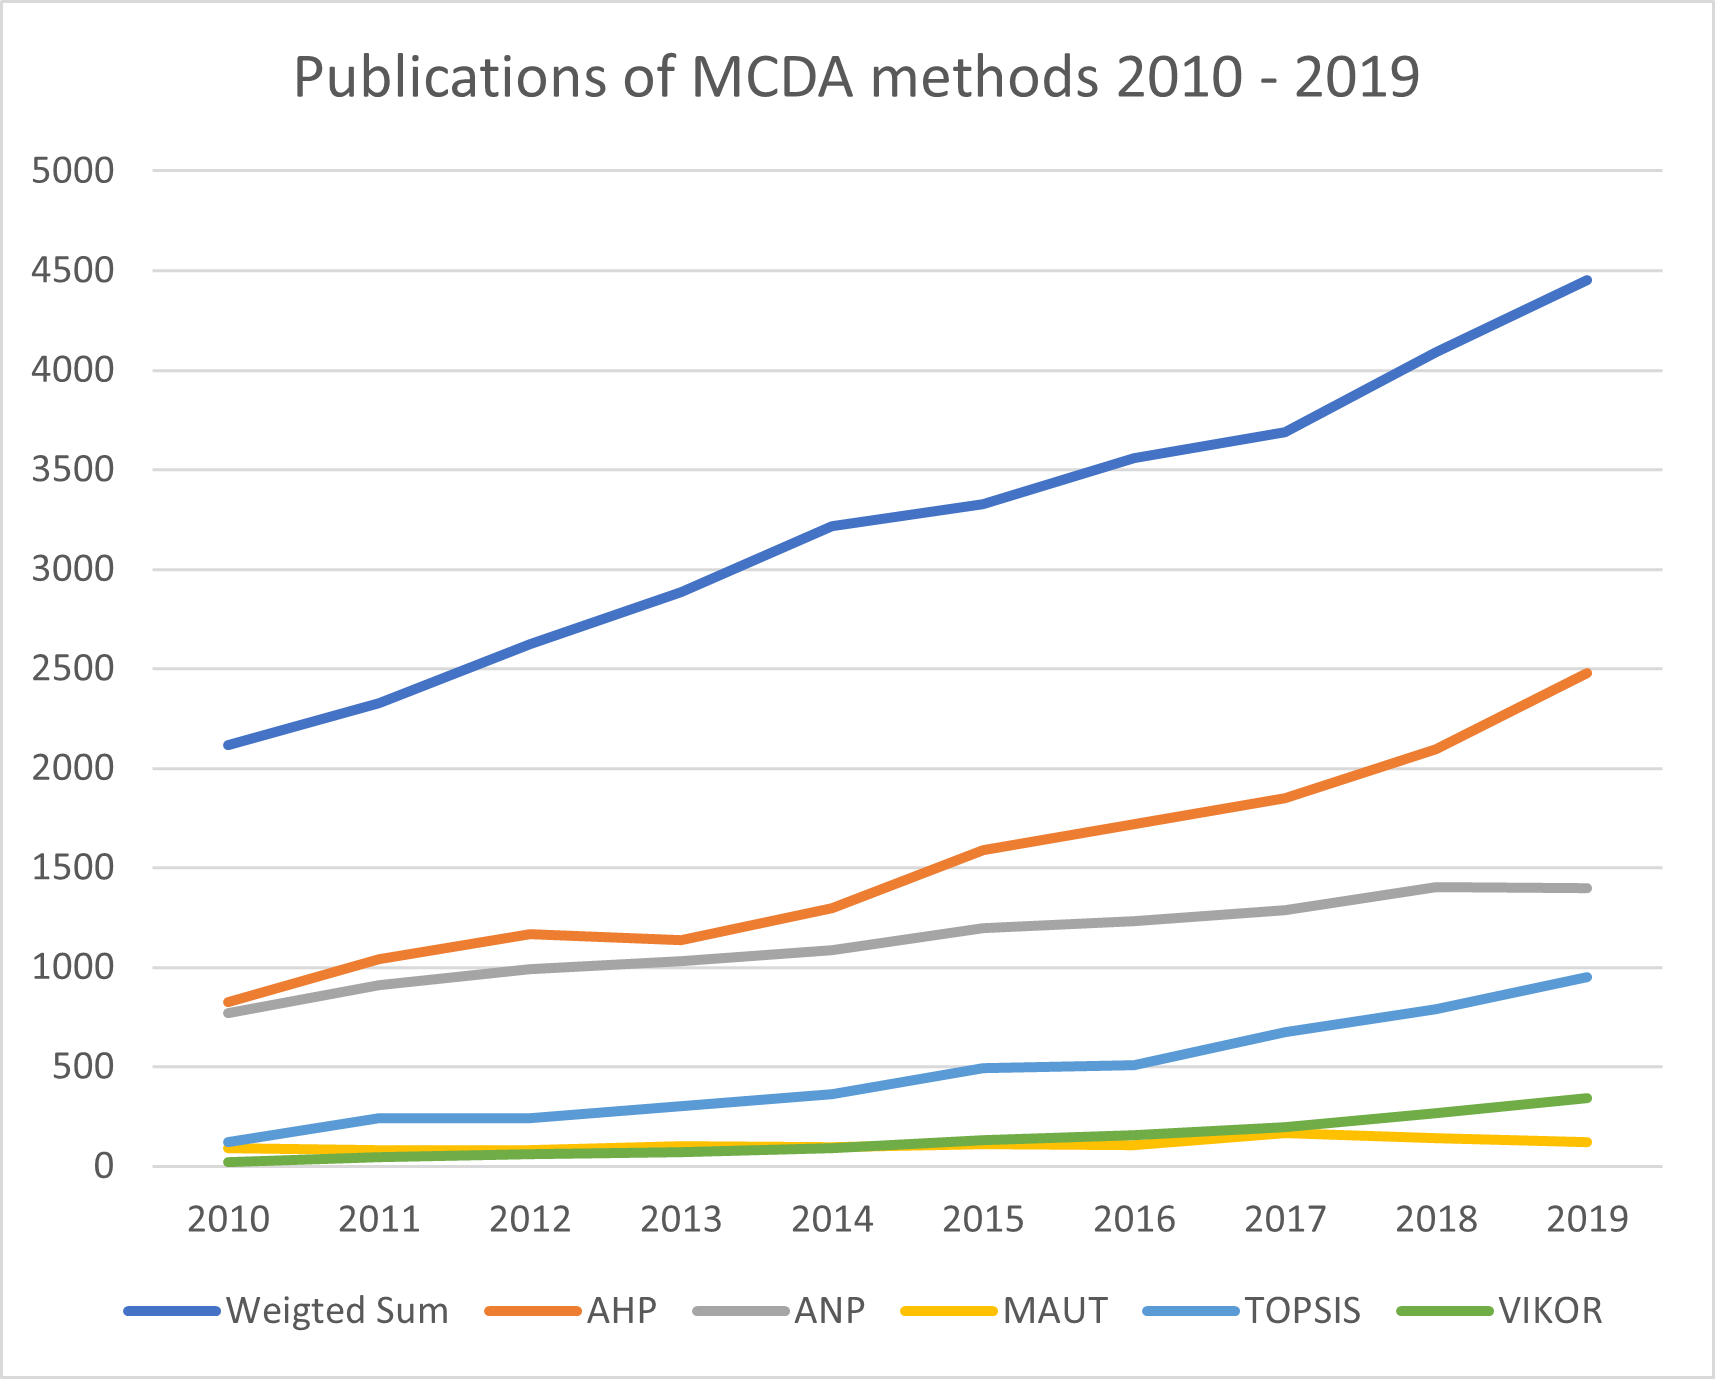
\includegraphics[width=9.5cm]{LUBS5308M Week03 Img001 - MCDA Methods}
	\centering
	\caption{Research outputs showing growing popularity of different MCDA techniques. (Source: Module Learning Material, Week 3)}
    \end{figure}

As the name implies, MCDA allows you to consider multiple conflicting criteria and decide on the best option using different types of information. 
Decisions are incredibly important in industry, especially decisions related to product development.\\
In the following sections, we will understand AHP and TOPSIS one by one with examples.
\section{Analytical Hierarchy Process}
 AHP is a pairwise comparison method, which is an approach to MCDA, in which we compare each alternative/criterion head-to-head with all the other alternatives/criteria and it is up to the decision maker to choose the best comparison.\\
 Saaty also proposed the use of 1-9 scale for AHP when comparing criterion and alternatives in order to facilitate the comparisons and convert qualitative comparisons to a quantitative scale.\\
 It was given by \href{https://en.wikipedia.org/wiki/Thomas_L._Saaty}{Prof. Thomas Saaty} in 1970. \\
\begin{table}[h]
\setlength{\arrayrulewidth}{0.25mm}
\setlength{\tabcolsep}{18pt}
% \renewcommand{\arraystretch}{0.25}
\begin{tabular}{ |p{1cm}|p{3cm}|p{5cm}|  }
\hline
\textbf{Scale}& \textbf{Verbal Expression} &\textbf{Explanation} \\
\hline
1 & Equal Importance & Two criterion are considered to be \textbf{equally} important. \\
\hline
3 & Moderate Importance & One criteria is \textbf{slightly} preferred over the other. \\
\hline
5 & Strong Importance & One criteria is \textbf{strongly} preferred over the other. \\
\hline
7 & Very Very Strong Importance & One criteria is favoured \textbf{very strongly} over another. \\
\hline
9 & Extreme Importance & One criteria is favoured over another with highest affirmation. \\
\hline
\end{tabular}
\caption{\label{tab:table1}1 - 9 Scale used for AHP.}
\end{table} \\
Suppose we are given two critera, $C_j$ and $C_k$. We will first calculate the relative importance of the criteria in decision making. Suppose $a_{j,k}$ is the value captured from the semantic scale(\ref{tab:table1}). The relative importance of $C_k$ over $C_j$ is defined as its reciprocal, i.e, $a_{k,j}$ = 1 / $a_{j,k}$.
A reciprocal matrix {\em A} is then formed using $a_{j,k}$ for all \em j and \em k.
There are two approaches to elicit scores from the reciprocal matrix:
\begin{enumerate}[noitemsep]
    \item Eigenvector method
    \item Geometric mean method
\end{enumerate}
It has been generally agreed that the weights of criteria can be estimated by finding the principal eigenvector $\omega$ of matrix A: 
\begin{center}
{\em \large AW} = $\lambda_{max}\omega$.
\end{center}
Using similar procedures, the weights of alternatives with respect to each criterion are computed. Then, the overall weights of alternatives are computed using the weighted summation:
\begin{center}

\left( \begin{array}{cc} Overall\:Weight \\
of\:alternative\:i \end{array} \right) =\:\: $\sum_j$
\left( \begin{array}{c} Weight\:of\:alternative\:i\:with \\ respect\:to\: Cj\: X \:Weight\: of\: Cj\: \\ with\: respect\: to\: the\: goal \end{array} \right)

\end{center}
\end{document}
